% Appendix E -- the two studies that do not fit the twelve-subject benchmark:
% corpus-scale external validation, and the full personalisation sweep.
\section{Large-Scale Studies: Corpus Validation and Personalisation}
\label{app:largescale}

\subsection{External Validation at Corpus Scale}
\label{sec:metabonet}

% causalcgm-mt-provenance: fingerprint=bc8b1ec3d72b4329 smoke=false generated=2026-10-06T21:08:00
\begin{table*}[t]
\centering
\small
\setlength{\tabcolsep}{4pt}
\caption{MetaboNet benchmark at PH~=~30~min, 5-fold patient-wise cross validation over 1838 subjects from 11 source studies (AZT1D, BrisT1D, CTR3, DCLP3, DCLP5, Flair, IOBP2, Loop, PEDAP, ReplaceBG, T1D-UOM). Whole subjects are held out, so the protocol measures generalisation to an unseen individual; MetaboNet's own \texttt{is\_test} column is a within-subject temporal split and is not used here. OhioT1DM and HUPA-UCM are excluded from the corpus, since both are benchmarks reported elsewhere in this work. Values are means over folds.}
\label{tab:metabonet_comparison}
\resizebox{\ifdim\width>\linewidth\linewidth\else\width\fi}{!}{%
\begin{tabular}{lrrrrrrrrrrrr}
\toprule
Model & RMSE & MAE & MARD (\%) & Lag (min) & A+B (\%) & D+E ($n$) & Parkes A+B (\%) & PR-AUC & Se@5\% & Se@10\% & FAPD@5\% & Onset lead (min) \\
\midrule
cgm\_only & 23.38 & 16.08 & 11.37 & \textbf{22.0} & 98.55 & 2016 & 99.38 & 0.820 & 0.875 & 0.941 & 3.87 & \textbf{22.3} \\
fusion & \textbf{23.08} & \textbf{15.87} & \textbf{11.22} & 22.5 & \textbf{98.58} & \textbf{1970} & \textbf{99.40} & \textbf{0.822} & \textbf{0.875} & \textbf{0.942} & 3.58 & 22.3 \\
\bottomrule
\end{tabular}}
\end{table*}


\begin{figure*}[t]
  \centering
  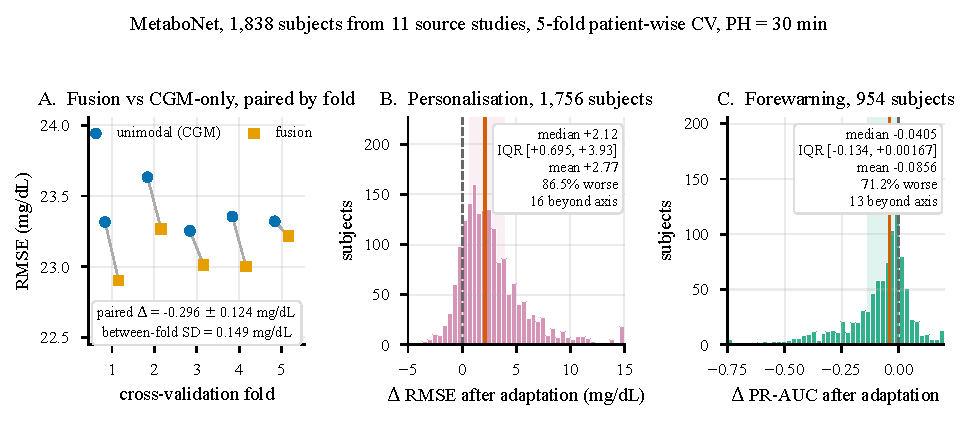
\includegraphics[width=\textwidth]{fig7_metabonet_corpus_scale.pdf}
  \caption{Corpus-scale external validation on MetaboNet,
  $\PH = \NumMetaboHorizon$~min. (A)~Fusion against the CGM-only model, paired
  by fold: both arms are trained on identical splits. (B)~Few-shot LoRA
  adaptation from a $\NumMetaboPersPrefixHours$-hour prefix, per held-out
  subject; positive is worse, the dashed line is no change, the shaded band the
  interquartile range. (C)~The same subjects' forewarning PR-AUC, over the
  $\NumMetaboPersPRAUCSubjects$ whose evaluation region contains hypoglycemia at
  all; negative is worse. Long tails are clipped to the axis with the clipped
  count stated, not dropped.}
  \label{fig:metabonet}
\end{figure*}

This appendix re-measures two OhioT1DM findings on MetaboNet~\citep{wolff2026metabonet},
a consolidated corpus of CGM studies stacked into one table: whether auxiliary fusion improves
on the CGM-only model, and whether few-shot personalisation from a one-day
prefix degrades the population model. $\NumMetaboSources$ source studies
contribute $\NumMetaboSubjects$ subjects. OhioT1DM and HUPA-UCM are excluded as
this paper's own benchmarks; ShanghaiT1DM contributes no window that clears the
gap and observability filters of invariants~I1--I2; and the SIESTA study, added
to the public release after our original analysis, is excluded so that the
corpus matches the one first analysed.

Most of these data were recorded under automated insulin delivery. In
$\NumMetaboCLStudies$ of the $\NumMetaboSources$ contributing studies the
released records come from automated insulin delivery systems, and these studies
supply $\NumMetaboCLSubjPct\%$ of the subjects; $\NumMetaboCLMixedStudies$
more mix automated and non-automated periods or participants, and
$\NumMetaboCLNoStudies$ used none (per-study classes and sources:
\texttt{manuscript/metabonet\_study\_design.json}). Not all of these studies
are trials: the largest source is an observational study of a community-built
system. In such data part of the insulin signal may reflect a controller
responding to glucose rather than an independent input.

\paragraph{The corpus contains this paper's benchmarks, and that is disqualifying.}
The release we analysed includes two of this paper's benchmarks, OhioT1DM and
HUPA-UCM:
all twelve Ohio subjects, including the CGM samples that fall inside the official
\emph{test} spans, every row labelled as training data. Fitting on the
consolidated corpus and reporting on either benchmark is training on the test
set, and the resulting metrics would improve rather than fail visibly.
OhioT1DM and HUPA-UCM are therefore dropped from the corpus by default and the
loader refuses them explicitly. A second hazard is quieter: subject
identifiers collide across source studies, so a bare identifier is not a subject
key and a patient-wise split built on one leaks a person across the fold
boundary. Keys are composite throughout.

\paragraph{Protocol.} Whole subjects are held out under
$\NumMetaboFolds$-fold patient-wise cross validation, so the question asked is
generalisation to an unseen individual. MetaboNet ships an \texttt{is\_test}
column, but it marks a \emph{within}-subject temporal split and answers the
other question; mixing rows from both into one table is the confusion
Section~\ref{sec:setup} refuses for OhioT1DM, and the same rule applies here.
Windowing the whole corpus at stride~1 would produce two orders of magnitude
more tensor data than the machine has memory for, so each subject contributes
at most $\NumMetaboCap$ windows, drawn as
contiguous blocks spread across the record rather than every $k$-th anchor.
Thinning by stride would sever every alarm episode at a sampling gap and empty
the lead-time and false-alarm metrics without emptying the table. That leaves
$\NumMetaboWindows$ windows at a hypoglycemia prevalence of
$\NumMetaboHypoPrev\%$, which is the floor the unimodal arm's
$\NumMetaboCGMPRAUC$ PR-AUC should be read against.

\paragraph{Fusion versus CGM-only.} The submitted version of this analysis
reported that the fusion arm landed on the unimodal baseline. That result was an
artefact: a defect in the per-window presence gate kept insulin and
carbohydrate channels, which carry no observation mask, from ever enabling the
fusion branch, so it opened only on windows carrying a masked wearable stream. With the gate corrected the
branch is active on $\NumMetaboFusionActiveMinPct$--$\NumMetaboFusionActiveMaxPct\%$
of test windows per fold. Fusion then lowers RMSE in all
$\NumMetaboFusionRMSEBetterFolds$ folds: the fold-paired difference is
$\NumMetaboFusionDeltaRMSE \pm \NumMetaboFusionDeltaRMSESD$~mg/dL, about
$\NumMetaboFusionEffectToSpread\times$ the between-fold spread of the CGM-only
arm ($\NumMetaboFoldSDRMSE$~mg/dL). It lowers false alarms per day (fold-paired
difference $\NumMetaboFusionDeltaFAPD \pm \NumMetaboFusionDeltaFAPDSD$; lower in
$\NumMetaboFusionFAPDBetterFolds$ of $\NumMetaboFolds$ folds). Its PR-AUC gain,
$\NumMetaboFusionDeltaPRAUC \pm \NumMetaboFusionDeltaPRAUCSD$, is negligible, and
its effect on Clarke zone D/E counts is not resolved
($\NumMetaboFusionDeltaDE \pm \NumMetaboFusionDeltaDESD$; fewer in
$\NumMetaboFusionDEBetterFolds$ of $\NumMetaboFolds$ folds). This replicates the
direction of the OhioT1DM point-accuracy gain at a smaller magnitude. Because
cross-validation folds share training subjects, the per-fold differences are not
independent replicates, and we report their spread and sign counts rather than a
significance test. In the automated-insulin-delivery studies, part of what the
insulin channels carry may be the controller's own response to falling glucose,
so this gain should be read as what the recorded treatment channels add to CGM,
not as evidence about insulin as an independent physiological input. Lead
time in Table~\ref{tab:metabonet_comparison} is measured to onset, as in
Section~\ref{sec:results}.

\paragraph{The personalisation failure replicates, in the regime we said was
open.} Section~\ref{sec:personalisation} cannot test adaptation to a subject the
population model has never seen, which is the regime few-shot personalisation is
usually claimed for. Patient-wise cross validation is that protocol. It scores
$\NumMetaboPersSubjects$ of the $\NumMetaboSubjects$ corpus subjects: the paired
design needs a full adaptation prefix, one embargo, and at least 50 evaluation
windows after it, all from one subject's kept windows, and $\NumMetaboPersSkipped$ records are too
short to supply all three. They are skipped rather than scored on a truncated
prefix, an exclusion that turns on record length rather than on the subject's
glycemia and is applied before any adaptation runs. Each of the
$\NumMetaboPersSubjects$ is adapted from a
$\NumMetaboPersPrefixHours$-hour prefix of its own record (a median of
$\NumMetaboPersAdaptWindows$ windows) with LoRA at rank~$\NumMetaboPersRank$,
$\NumMetaboPersTrainable$ trainable parameters, and scored on its own
post-embargo region. The held-out test rows themselves cannot be used, because
under this protocol they contain the prefix the adaptation was fitted on. Adaptation costs $\NumMetaboPersDeltaRMSE$~mg/dL of RMSE on average; the
median subject loses $\NumMetaboPersMedianDeltaRMSE$~mg/dL, the interquartile
range $[\NumMetaboPersDeltaRMSEQOne, \NumMetaboPersDeltaRMSEQThree]$ lies
entirely above zero, and $\NumMetaboPersWorsePct\%$ of subjects are worse after
adapting than before. Only $\NumMetaboPersImproved$ of
$\NumMetaboPersSubjects$ improve (Figure~\ref{fig:metabonet}B). The forewarning
task degrades too, on a smaller base: PR-AUC is undefined for a subject
whose evaluation region contains no hypoglycemia at all, so the mean change of
$\NumMetaboPersDeltaPRAUC$ is over the $\NumMetaboPersPRAUCSubjects$ subjects
where both sides are defined, $\NumMetaboPersPRAUCWorsePct\%$ of whom are worse
(Figure~\ref{fig:metabonet}C).
The sign matches OhioT1DM's $\NumPersLoRAFourRMSEDelta$~mg/dL, at
$\NumMetaboPersOhioPct\%$ of its magnitude. Here the adaptation data are
genuinely new to the population model, which the OhioT1DM design could not
ensure. The adaptation recipe is unchanged, however: a fixed step budget with no
held-out early stopping. This result therefore shows that this recipe degrades
unseen subjects too; it does not separate scarce data from over-adaptation as
the cause.

\paragraph{What this appendix does not establish.} One seed, one horizon
($\PH = \NumMetaboHorizon$~min), one adapter, one prefix length. The per-subject
window cap makes a long record contribute no more than a short one. The tabular
and classical baselines of Section~\ref{sec:baselines} were not re-fitted at this
scale; the only external reference is persistence at
$\NumMetaboPersistRMSE$~mg/dL.

\subsection{Few-Shot Personalisation: A Negative Result}
\label{sec:personalisation}

The OhioT1DM protocol is temporal and \emph{within} patient, which makes
per-subject adaptation the natural question to ask of it. We adapt the
population model to each of $\NumPersSubjects$ subjects from a
$\NumPersPrefixHours$-hour prefix of that subject's own training file, separated
from every evaluation window by the embargo of invariant~I5, and compare before
and after on \emph{identical} windows. Those windows are the official test file
alone. The prefix--embargo geometry separates the \emph{adaptation} data from the
evaluation data, but it says nothing about the \emph{population} model, which was
fitted on the training file the prefix is drawn from; scoring on the remainder of
that file as well would leave most of the evaluation region in-sample for the
zero-shot arm the deltas are measured against. Restricting to the released
testing windows costs roughly half the hypoglycemic events and is the only set
disjoint from both the fit and the model-selection split. Six arms are tested: no adaptation and five adapted modes,
BatchNorm statistic recalibration~\citep{schneider2020improving}, LoRA~\citep{hu2022lora} at ranks 4 and 8 with
an L2-SP anchor~\citep{xuhong2018explicit}, head-only fine-tuning, and full
fine-tuning. Because five adapted modes are tested at each prefix length, $p$-values are
Holm--Bonferroni adjusted~\citep{holm1979simple} within that family.

At the default budget of $\NumPersDefaultSteps$ gradient steps and the
$\NumPersPrefixHours$-hour prefix (Table~\ref{tab:personalization}), every
adapted mode makes the model worse on RMSE and PR-AUC, and the effects are not
marginal. At $\PH = 30$~min, BatchNorm adaptation costs $\NumPersBNAdaptRMSEDelta$~mg/dL RMSE
($p_{\text{Holm}} = \NumPersBNAdaptRMSEP$) and
$\NumPersBNAdaptPRAUCDelta$ PR-AUC; LoRA at rank~4 costs
$\NumPersLoRAFourRMSEDelta$~mg/dL and $\NumPersLoRAFourPRAUCDelta$ PR-AUC; full
fine-tuning costs $\NumPersFullRMSEDelta$~mg/dL and
$\NumPersFullPRAUCDelta$ PR-AUC. RMSE improved for
$\NumPersLoRAFourRMSEImproved$ of $\NumPersSubjects$ subjects under LoRA.
False-alarm rates are not reported for the adapted models: alarm thresholds are
fitted on calibration data, and this protocol has none for a per-subject model.

Two diagnostics describe the damage. First, it grows with the adaptation
budget: LoRA at rank~4 changes RMSE by $\NumPersLoRAStepsTenDelta$~mg/dL after
ten gradient steps and $\NumPersLoRAStepsTwoHundredDelta$ after two hundred.
That is the signature of over-adaptation to the prefix, and no mode here uses
held-out early stopping to prevent it. Second, BatchNorm adaptation, which
recomputes running statistics on the prefix and updates no weights, also
degrades the model: by $\NumPersBNPrefixSixDelta$~mg/dL from a six-hour prefix
(over $\NumPersPrefixSixN$ subjects; the other prefix lengths use all
$\NumPersPrefixTwentyFourN$),
$\NumPersBNPrefixTwentyFourDelta$ from twenty-four hours and
$\NumPersBNPrefixFortyEightDelta$ from forty-eight. Replacing population
activation statistics with one subject's is therefore harmful in itself, and the
cost stops shrinking after a day of data, which a pure estimation-noise account
would not predict. Head-only fine-tuning, by contrast, keeps improving with
prefix length ($\NumPersHeadPrefixSixDelta \to
\NumPersHeadPrefixFortyEightDelta$~mg/dL from six to forty-eight hours, the
six-hour value over $\NumPersPrefixSixN$ subjects and the rest over
$\NumPersPrefixTwentyFourN$) without reaching zero.

These diagnostics do not isolate a single cause. Scarce adaptation data,
over-adaptation under a fixed step budget, and the loss of population
statistics are all consistent with them, and the design cannot separate them:
on OhioT1DM the prefix lies inside the population model's own training split, so
adaptation adds no new information.

\begin{table*}[t]
\centering
\small
\setlength{\tabcolsep}{4pt}
\caption{Few-shot personalisation on OhioT1DM, PH = 30 min, 24 h adaptation prefix, 12 subjects. $\Delta$ is the paired per-subject change from the zero-shot population model on identical evaluation windows; $p$ is a paired $t$-test with Holm--Bonferroni adjustment across modes. The zero-shot baseline reads 18.84~mg/dL here against 18.97~mg/dL in Table~\ref{tab:sota_ph30}: the same checkpoint on the same 28,335 windows, aggregated differently. This table averages the 12 per-subject RMSEs, which is the quantity the paired tests are computed on; Table~\ref{tab:sota_ph30} pools the residuals across all windows. Weighting these rows by their window counts recovers the pooled RMSE exactly (18.968 against 18.97). PR-AUC does not decompose this way: it is a rank statistic over the pooled residuals, so the per-subject mean (0.790, sd 0.145, range 0.566--0.954 across the 12 subjects) is a different quantity from the pooled 0.870 and is not recoverable from it by reweighting. The paired tests are computed on the per-subject values reported here.}
\label{tab:personalization}
\resizebox{\ifdim\width>\linewidth\linewidth\else\width\fi}{!}{%
\begin{tabular}{lrrrrrrrrr}
\toprule
Adaptation & RMSE & $\Delta$ RMSE & $p_{\mathrm{Holm}}$ & PR-AUC & $\Delta$ PR-AUC & $p_{\mathrm{Holm}}$ & FAPD@5\% & $\Delta$ FAPD@5\% & $p_{\mathrm{Holm}}$ \\
\midrule
none & \textbf{18.844} & \textbf{+0.000} & -- & \textbf{0.790} & \textbf{+0.000} & -- & -- & -- & -- \\
bn\_adapt & 19.887 & +1.043 & 0.008 & 0.733 & -0.057 & 0.063 & -- & -- & -- \\
lora (r=4) & 21.678 & +2.834 & 0.000 & 0.686 & -0.105 & 0.063 & -- & -- & -- \\
lora (r=8) & 21.366 & +2.522 & 0.000 & 0.678 & -0.112 & 0.036 & -- & -- & -- \\
head\_only & 19.545 & +0.701 & 0.022 & 0.734 & -0.056 & 0.033 & -- & -- & -- \\
full & 22.826 & +3.982 & 0.000 & 0.697 & -0.094 & 0.006 & -- & -- & -- \\
\bottomrule
\end{tabular}}
\end{table*}

\begin{table*}[t]
\centering
\small
\setlength{\tabcolsep}{4pt}
\caption{Adaptation budget: mean paired $\Delta$RMSE (mg/dL) as a function of the number of gradient steps, at a 24 h prefix and PH = 30 min. For LoRA at both ranks the damage grows with every increase in the budget; head-only fine-tuning is not monotone.}
\label{tab:step_budget}
\resizebox{\ifdim\width>\linewidth\linewidth\else\width\fi}{!}{%
\begin{tabular}{lrrrrr}
\toprule
Adaptation & 10 steps & 25 steps & 50 steps & 100 steps & 200 steps \\
\midrule
lora (r=4) & -0.018 & +0.378 & +1.078 & +1.873 & +2.834 \\
lora (r=8) & -0.055 & +0.240 & +0.886 & +1.726 & +2.522 \\
head\_only & \textbf{-0.221} & \textbf{-0.287} & \textbf{-0.111} & \textbf{+0.225} & \textbf{+0.701} \\
\bottomrule
\end{tabular}}
\end{table*}


The natural explanation is within-subject drift. A short prefix would then be an
unrepresentative sample of the subject's \emph{own} later distribution: glucose
dynamics move within a person across weeks, so the opening day of a record is a
biased estimate of the month that follows, and adapting to it pulls the model
away from the evaluation period rather than toward it. On this cohort the
opening prefix ends a median of $\NumPosOpeningGapDays$~days before the first
scored window, which is ample room for such a decoupling.

\paragraph{The drift explanation is testable, and it fails.} If staleness were
the mechanism, a prefix drawn from the evaluation window's own temporal
neighbourhood should not fail the same way. We therefore add a
\emph{prefix-position} control: the same $\NumPersPrefixHours$ hours, the same
subjects, the same evaluation windows, the same adapter and the same step
budget, but taken from the \emph{end} of the training file so that the prefix
closes exactly one embargo ($\NumPosRecentGapMin$~minutes) before the first
scored window. Only the distance between the adaptation data and the scored data
changes. The sweep records where each prefix lies relative to the population
model's fit and model-selection rows. All $\NumPosOpeningAdaptWindowsTotal$ adaptation
windows of the opening prefix, summed over subjects, lie in the fit rows. None of
the $\NumPosRecentAdaptWindowsTotal$ recent-prefix windows lies in the fit rows
($\NumPosRecentAdaptInFit$) or in the model-selection rows
($\NumPosRecentAdaptInVal$). The contrast therefore changes recency and also
whether the adaptation windows were seen in training; it does not separate the two.

\begin{table*}[t]
\centering
\small
\setlength{\tabcolsep}{4pt}
\caption{Adaptation prefix position at a 24 h prefix, PH = 30 min. Both arms use the same subjects, evaluation windows, adapter, step budget and prefix length; they differ only in how far the prefix sits from the windows being scored. The opening prefix ends a median of 44~days before the first scored window; the recent prefix ends 185~min before it, which is the embargo itself. No column of paired differences is significant, and no arm becomes an improvement over zero-shot under either position. Negative $\Delta$RMSE and positive $\Delta$PR-AUC are better.}
\label{tab:prefix_position}
\resizebox{\ifdim\width>\linewidth\linewidth\else\width\fi}{!}{%
\begin{tabular}{lrrrrrrrr}
\toprule
Adaptation & $\Delta$RMSE open & $\Delta$RMSE recent & rec$-$open & $p_{\mathrm{Holm}}$ & $\Delta$PR-AUC open & $\Delta$PR-AUC recent & rec$-$open & $p_{\mathrm{Holm}}$ \\
\midrule
none & +0.000 & +0.000 & +0.000 & -- & +0.000 & +0.000 & +0.000 & -- \\
bn\_adapt & +1.043 & +1.521 & +0.478 & 0.977 & -0.057 & -0.046 & +0.011 & 1.000 \\
lora (r=4) & +2.834 & +3.754 & +0.920 & 0.888 & -0.105 & -0.154 & -0.049 & 1.000 \\
lora (r=8) & +2.522 & +3.313 & +0.791 & 0.699 & -0.112 & -0.154 & -0.042 & 1.000 \\
head\_only & +0.701 & +1.566 & +0.865 & 0.888 & -0.056 & -0.041 & +0.015 & 1.000 \\
full & +3.982 & +4.209 & +0.227 & 0.977 & -0.094 & -0.196 & -0.102 & 0.412 \\
\bottomrule
\end{tabular}}
\end{table*}


Recency does not rescue adaptation. At the default step budget, every adapted
mode still raises RMSE from a recent prefix, and significantly so: BatchNorm adaptation costs
$\NumPosRecentBNAdaptRMSEDelta$~mg/dL ($p_{\text{Holm}} =
\NumPosRecentBNAdaptRMSEP$), LoRA at rank~4 $\NumPosRecentLoRAFourRMSEDelta$
($p_{\text{Holm}} = \NumPosRecentLoRAFourRMSEP$) and full fine-tuning
$\NumPosRecentFullRMSEDelta$ ($p_{\text{Holm}} = \NumPosRecentFullRMSEP$). The
paired recent-minus-opening differences are null throughout, and no mode does
better from the recent prefix: every difference is positive, the smallest being
$\NumPosBestDiffRMSE$~mg/dL (raw $p = \NumPosBestDiffP$). For LoRA at rank~4 the
95\% confidence interval of the difference,
$[\NumPosDiffLoRAFourRMSECILow, \NumPosDiffLoRAFourRMSECIHigh]$, straddles zero;
the smallest Holm-adjusted $p$ across all modes is $\NumPosMinDiffPHolm$. Head-only
fine-tuning is nominally \emph{worse} from the recent prefix
($\NumPosDiffHeadOnlyRMSE$~mg/dL), and full fine-tuning is worse on forewarning
($\NumPosDiffFullPRAUC$ PR-AUC). Moving the adaptation data
$\NumPosOpeningGapDays$~days closer to the windows being scored changes
essentially nothing.

The prefix-position control therefore gives no support to drift as the
explanation: a recent prefix degrades the model as much as an opening one, within
the precision twelve subjects allow.

The reading we can support is narrow. With this recipe (a prefix of at most 48
hours, no held-out early stopping), at the default step budget and the
$\NumPersPrefixHours$-hour prefix every adapted mode degrades the population
model on OhioT1DM, and shipping the population model unchanged is the better of
those configurations. Very short head-only budgets are the exception on RMSE
(Table~\ref{tab:step_budget}): $\NumPersHeadOnlyStepsTenDelta$~mg/dL after ten steps,
$\NumPersHeadOnlyStepsTwentyFiveDelta$ after twenty-five and
$\NumPersHeadOnlyStepsFiftyDelta$ after fifty, with $\NumPersHeadStepsTenImproved$ of
$\NumPersSubjects$ subjects improving at ten steps. The ten-step interval,
$[\NumPersHeadStepsTenCILow, \NumPersHeadStepsTenCIHigh]$ with $p =
\NumPersHeadStepsTenP$, is unadjusted: the step-budget cells carry no multiplicity
correction, so we do not call it significant. Mean PR-AUC does not improve at any
budget for any adapter in that table. Whether longer prefixes, genuinely new adaptation
data or held-out early stopping change that remains open. A held-out-subject
protocol, the regime few-shot personalisation is usually claimed for, is tested
in Appendix~\ref{sec:metabonet}: on $\NumMetaboPersSubjects$ unseen subjects the
same adapter and prefix length cost $\NumMetaboPersDeltaRMSE$~mg/dL.
